\documentclass[11pt]{article}            % Report class in 11 points
\parindent0pt  \parskip10pt             % make block paragraphs
\usepackage{graphicx}
\usepackage{listings}
\usepackage[document]{ragged2e}
\usepackage{float}
\newcommand\tab[1][1cm]{\hspace*{#1}}
\graphicspath{ {images/} }
\usepackage{graphicx} %  graphics header file
\begin{document}
\begin{titlepage}
    \centering
  \vfill
    
\includegraphics[width=8cm]{uni_logo.png} \\ 
	\vskip2cm
    {\bfseries\Large
	Data Structures  \& Algorithms \\ (CS09203)\\
	
	\vskip2cm
	Lab Report 
	 
	\vskip2cm
	}    

\begin{center}
\begin{tabular}{ l l  } 

Name: & Muhammad Umer \\ 
Registration \#: & CSU-F16-104 \\ 
Lab Report \#: & 06 \\ 
 Dated:& 14-05-2018\\ 
Submitted To:& Mr. Usman Ahmed\\ 

 %\hline
\end{tabular}
\end{center}
    \vfill
    The University of Lahore, Islamabad Campus\\
Department of Computer Science \& Information Technology
\end{titlepage}


    
    {\bfseries\Large
\centering
	Experiment \# 1 \\

Create a C++ program to implement Doubly Linked List and Travers it\\
	
	}    
 \vskip1cm
 \textbf {Objective}\\  To understand and implement the DOubly Link List with basic Insertion, and Traversal.
 
 \textbf {Software Tool} \\
1. Sublime Text Editor\\
2. Dev C++\\
3. Window 7 (32 Bit)\\

\section{Theory }              
\justify A doubly-linked list is a linked data structure that consists of a set of sequentially linked records called nodes. Each node contains two fields, called links, that are references to the previous and to the next node in the sequence of nodes.\\~\\
 A Doubly Linked List (DLL) contains an extra pointer, typically called previous pointer, together with next pointer and data which are there in singly linked list.\\~\\
\begin{figure}[H]
\centering
  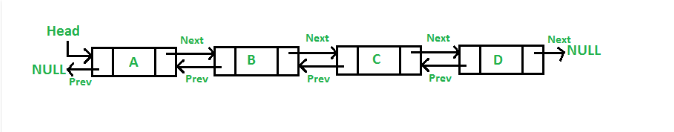
\includegraphics[width=12cm,height=6cm,keepaspectratio]{5.png}    
\end{figure}
\section{Task}  
\subsection{Procedure: Task 1 Insertion at the start}

In this Doubly Linked List user can insert integer type of the data and the data will always be inserted in the start of the list.  

\begin{lstlisting}[language=C++]

 
void insert(node* newNode){
	node* last_node = (node*)malloc(sizeof(node));
	last_node = head;
	head = newNode;
	newNode -> pre = NULL;
	newNode -> next = last_node;
	return;
}

Output:
\end{lstlisting}
Please see Figure 1 for output

\subsection{Procedure: Task 2 Traverse}     

\begin{lstlisting}[language=C++]
void display(){
	node* newNode = (node*)malloc(sizeof(node));
	newNode = head;
	cout<<"\n\nData in the list\n\n";
	while(newNode != NULL){
		cout<<newNode -> data<<" ";
		newNode = newNode -> next;
	}
	cout<<"\n\nPress any key to continue..";
	getch();
	return;
}

Output: 
\end{lstlisting}
Please see Figure 2 for output

\textbf{Source Code} \\
https://goo.gl/ccBvqK

\begin{figure}[b!]
\centering
  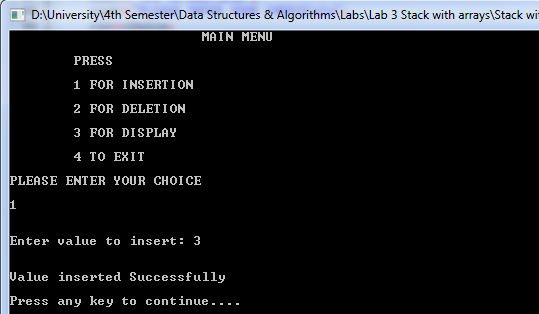
\includegraphics[width=12cm,height=6cm,keepaspectratio]{1.png}
\caption{Inserting in the list}
\label{Figure:1}    
\end{figure}

\begin{figure*}
\centering
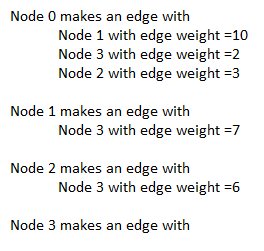
\includegraphics[width=12cm,height=6cm,keepaspectratio]{2.png}
\caption{Displaying after insertion}
\label{Figure:2}    
\end{figure*}


\section{Conclusion}
A Doubly linked list is a linear data structure where each element is a separate object. Each element is called as a node, that contains three item - the data, a reference to the previous node, and a reference to the next node. The last node has a reference to null. The entry point into a Doubly linked list is same as the simple linked list called the head of the list. A Doubly linked list is a dynamic data structure. The number of nodes in a list is not fixed and can grow and shrink on demand.\\~\\

\tab[6cm] \noindent\rule{6cm}{0.4pt}\\
\tab[6cm] (Concerned Teacher/Lab Engineer)


 
\end{document}                          % The required last line
